\documentclass[aspectratio=169, xcolor=dvipsnames]{beamer}

% Packages
\usepackage[utf8]{inputenc}
\usepackage{graphicx}
\usepackage{colortbl} % rowcolor support for tables
\usepackage{tabularx} % flexible tables
\usepackage{tikz}
\usepackage{amsmath}
\usetikzlibrary{fadings}
\usepackage{amssymb}
\usepackage{xcolor}
\usepackage{hyperref}
\usepackage{fontawesome5}
\usepackage{multicol}
\usetikzlibrary{positioning, fit, arrows.meta} % For TikZ positioning
\usepackage{tabularx} % For tabular environment in nodes
\usepackage{listings}
\usetikzlibrary{calc}

% TikZ Libraries
\usetikzlibrary{shapes, arrows, positioning, fit, shadows, calc}

% Custom Colors
\definecolor{Primary}{RGB}{255, 152, 0}       % Orange
\definecolor{Secondary}{RGB}{41, 88, 255}     % Blue
\definecolor{Accent}{RGB}{76, 175, 80}        % Green
\definecolor{DarkBg}{RGB}{30, 30, 30}         % Dark Background
\definecolor{LightBg}{RGB}{240, 240, 240}     % Light Background
\definecolor{Warning}{RGB}{255, 87, 34}       % Red-Orange

% Theme Customization
\usetheme{Madrid}
\usecolortheme{default}

% Custom Color Scheme
\setbeamercolor{structure}{fg=Primary}
\setbeamercolor{alerted text}{fg=Warning}
\setbeamercolor{block title}{bg=Primary, fg=white}
\setbeamercolor{block body}{bg=Primary!10, fg=black}
\setbeamercolor{title}{fg=Primary}
\setbeamercolor{subtitle}{fg=Secondary}
\setbeamercolor{frametitle}{bg=Primary, fg=white}
\setbeamercolor{section in toc}{fg=Primary}

% Custom Footer
\setbeamertemplate{footline}{
    \hbox{%
        \begin{beamercolorbox}[wd=0.5\paperwidth,ht=2.25ex,dp=1ex,left]{title in head/foot}%
            \usebeamerfont{title in head/foot}\hspace*{2ex}\insertshortauthor
        \end{beamercolorbox}%
        \begin{beamercolorbox}[wd=0.5\paperwidth,ht=2.25ex,dp=1ex,right]{date in head/foot}%
            \usebeamerfont{date in head/foot}\insertframenumber{} / \inserttotalframenumber\hspace*{2ex}
        \end{beamercolorbox}}%
    \vskip0pt%
}

% Title Page Style
\setbeamertemplate{title page}{
    \begin{tikzpicture}[remember picture, overlay]
        % Background image
        \node[anchor=center] at (current page.center) {
            \IfFileExists{imagebackground.png}{%
                \includegraphics[width=\paperwidth,height=\paperheight]{imagebackground.png}%
            }{%
                \includegraphics[width=\paperwidth,height=\paperheight]{background.png}%
            }
        };
        
        % Dark overlay for text contrast
        \fill[black, opacity=0.7] (current page.south west) rectangle (current page.north east);
    \end{tikzpicture}
    \centering
    
    % Logo (with fallback)
    \IfFileExists{app-logo.png}{%
        \includegraphics[width=0.15\textwidth]{app-logo.png}%
    }{%
        \IfFileExists{app-logo.png}{%
            \includegraphics[width=0.15\textwidth]{app-logo.png}%
        }
    }\\[0.15cm]
    
    % Title with white text for visibility
    {\LARGE \textbf{\textcolor{white}{PICK MY DISH}}}\\[0.2cm]
    {\Large \textcolor{white}{\textit{Your Personal Cooking Companion}}}\\[0.3cm]
    
    % Value bullets with white text
    {\normalsize \textcolor{white}{\textbullet\ Time-aware \hspace{0.4cm} \textbullet\ Mood-based \hspace{0.4cm} \textbullet\ Ingredient-aware}}\\[.7cm]
    
    % Content box with gradient background
    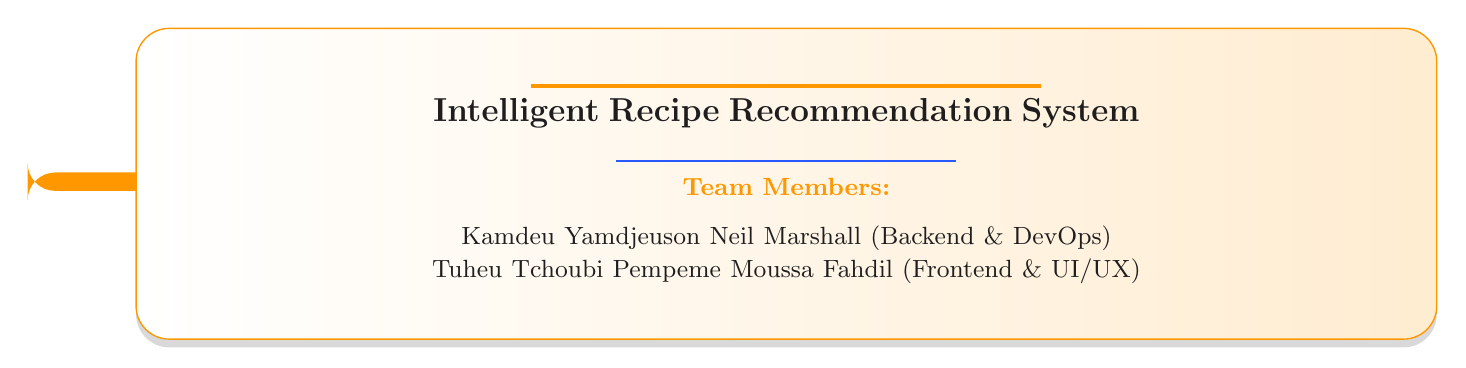
\begin{tikzpicture}
        % Decorative accent bar on top
        \node[fill=Primary, minimum width=0.8\paperwidth, minimum height=0.15cm, rounded corners=10pt, anchor=north] at (0.2, 0.15) {};
        
        % Main gradient box
        \node[
            left color=white, 
            right color=Primary!18,
            draw=Primary,
            line width=0.5pt,
            rounded corners=12pt,
            inner sep=20pt,
            text width=0.7\paperwidth,
            drop shadow={shadow xshift=0pt, shadow yshift=-3pt, opacity=0.3}
        ] at (1.20,0) {
            \centering
            % Decorative line
            \textcolor{Primary}{\rule{0.3\paperwidth}{1.5pt}}
            
            {\large \textcolor{DarkBg}{\textbf{Intelligent Recipe Recommendation System}}}\\[0.1cm]
            
            % Decorative separator
            \textcolor{Secondary}{\rule{0.2\paperwidth}{0.8pt}}
            
            {\small \textcolor{Primary}{\textbf{Team Members:}}}\\[0.2cm]
            {\small \textcolor{DarkBg}{Kamdeu Yamdjeuson Neil Marshall (Backend \& DevOps)}}\\
            {\small \textcolor{DarkBg}{Tuheu Tchoubi Pempeme Moussa Fahdil (Frontend \& UI/UX)}}
            
        };
    \end{tikzpicture}
}

% Content Page Style
\setbeamertemplate{frametitle}{
    \begin{beamercolorbox}[sep=0.3cm,wd=\paperwidth,ht=0.8cm]{frametitle}
        \textbf{\insertframetitle}
    \end{beamercolorbox}
}

\setbeamertemplate{background}{
    \begin{tikzpicture}[remember picture, overlay]
        % Main gradient background
        \fill[top color=white, bottom color=Primary!5] 
            (current page.south west) rectangle (current page.north east);
        
        % Decorative circles pattern
        \foreach \i in {1,...,20} {
            \fill[Primary!3, rotate around={20*\i:(current page.center)}] 
                (current page.center) ellipse[x radius=0.2\paperwidth, y radius=0.4\paperheight];
        }
        
        % Geometric accent top-right
        \fill[Primary!10, rounded corners=10pt] 
            ($(current page.north east)+(-3cm,-1.5cm)$) rectangle 
            ($(current page.north east)+(-0.5cm,-0.5cm)$);
        \fill[Secondary!15, rotate=45] 
            ($(current page.north east)+(-2cm,-2cm)$) rectangle 
            ($(current page.north east)+(-1.5cm,-3cm)$);
        
        % Geometric accent bottom-left  
        \fill[Secondary!10, rounded corners=10pt] 
            ($(current page.south west)+(0.5cm,0.5cm)$) rectangle 
            ($(current page.south west)+(3cm,1.5cm)$);
        \fill[Primary!15, rotate=45] 
            ($(current page.south west)+(1.5cm,1.5cm)$) rectangle 
            ($(current page.south west)+(2cm,3cm)$);
        
        % Top gradient bar (under title)
        \fill[Primary, opacity=0.1, path fading=east] 
            (current page.north west) ++(0,-1.8cm) rectangle 
            ($(current page.north east)+(0,-2cm)$);
        
        % Decorative dots pattern
        \foreach \x in {0.1,0.2,...,0.9} {
            \foreach \y in {0.2,0.4,0.6,0.8} {
                \fill[Accent!30] ($(current page.west)!\x!(current page.east)$) 
                    ++(0,-\y*\paperheight) circle (0.5pt);
            }
        }
        
        % Corner decorative elements
        \begin{scope}[rotate around={45:($(current page.north east)+(-0.8cm,-0.8cm)$)}]
            \draw[Primary!20, line width=2pt] 
                ($(current page.north east)+(-1.2cm,-1.2cm)$) -- 
                ($(current page.north east)+(-2cm,-2cm)$);
        \end{scope}
        
        \begin{scope}[rotate around={-45:($(current page.south west)+(0.8cm,0.8cm)$)}]
            \draw[Secondary!20, line width=2pt] 
                ($(current page.south west)+(1.2cm,1.2cm)$) -- 
                ($(current page.south west)+(2cm,2cm)$);
        \end{scope}
    \end{tikzpicture}
}

% Remove navigation symbols
\setbeamertemplate{navigation symbols}{}

% Font Settings
\usefonttheme{default}
\setbeamerfont{title}{series=\bfseries, size=\Large}
\setbeamerfont{subtitle}{series=\bfseries, size=\normalsize}
\setbeamerfont{frametitle}{series=\bfseries, size=\large}
\setbeamerfont{block title}{series=\bfseries}

\title{PICK MY DISH}
\subtitle{Intelligent Recipe Recommendation System}
\author{Group 01}
\date{January 2026}

\begin{document}

% ============================================================
% SLIDE 1: TITLE PAGE
% ============================================================
{%% scope background to this frame only

\begin{frame}[plain]
    \titlepage
\end{frame}
}%% end scoped background

% ============================================================
% SLIDE 2: THE PROBLEM & SOLUTION
% ============================================================
\begin{frame}{The Problem \& Our Solution}
    \vspace*{0.2cm}
    
    \begin{columns}[T]
        % PROBLEM COLUMN
        \column{0.48\textwidth}
        \centering
        
\begin{tikzpicture}
            % Header with icon
            \node[fill=Warning, text=white, minimum width=0.9\textwidth, 
                  minimum height=0.8cm, rounded corners=8pt, font=\bfseries\Large] 
                at (0,0) {\faExclamationTriangle~THE CHALLENGE};
        \end{tikzpicture}
        
        \vspace{0.3cm}
        
        \begin{tikzpicture}
            % Problem items with icons
            \node[draw=Warning, fill=Warning!8, thick, rounded corners=10pt,
                  minimum width=0.9\textwidth, minimum height=0.8cm,
                  label={[xshift=-2.5cm, Warning]\faUserClock}] (p1) at (0,0) 
                  {\textbf{Decision Fatigue}};
                  
            \node[draw=Warning, fill=Warning!8, thick, rounded corners=10pt,
                  minimum width=0.9\textwidth, minimum height=0.8cm,
                  label={[xshift=-2.5cm, Warning]\faMoneyBillWave}] (p2) at (0,-1.4) 
                  {\textbf{Limited Resources}};
                  
            \node[draw=Warning, fill=Warning!8, thick, rounded corners=10pt,
                  minimum width=0.9\textwidth, minimum height=0.8cm,
                  label={[xshift=-2.5cm, Warning]\faHourglassHalf}] (p3) at (0,-2.85) 
                  {\textbf{Time Constraints}};
                  
            \node[draw=Warning, fill=Warning!8, thick, rounded corners=10pt,
                  minimum width=0.9\textwidth, minimum height=0.8cm,
                  label={[xshift=-2.5cm, Warning]\faUserSlash}] (p4) at (0,-4.25) 
                  {\textbf{No Personalization}};
        \end{tikzpicture}
        
        % SOLUTION COLUMN  
        \column{0.48\textwidth}
        \centering
        
\begin{tikzpicture}
            % Header with icon
            \node[fill=Accent, text=white, minimum width=0.9\textwidth, 
                  minimum height=0.8cm, rounded corners=8pt, font=\bfseries\Large] 
                at (0,0) {\faLightbulb~OUR SOLUTION};
        \end{tikzpicture}
        
        \vspace{0.3cm}
        
        \begin{tikzpicture}
            % Solution items with icons
            \node[draw=Accent, fill=Accent!8, thick, rounded corners=10pt,
                  minimum width=0.9\textwidth, minimum height=0.8cm,
                  label={[xshift=-2.5cm, Accent]\faRobot}] (s1) at (0,0) 
                  {\textbf{AI Recommendations}};
                  
            \node[draw=Accent, fill=Accent!8, thick, rounded corners=10pt,
                  minimum width=0.9\textwidth, minimum height=0.8cm,
                  label={[xshift=-2.5cm, Accent]\faFilter}] (s2) at (0,-1.4) 
                  {\textbf{Smart Filtering}};
                  
            \node[draw=Accent, fill=Accent!8, thick, rounded corners=10pt,
                  minimum width=0.9\textwidth, minimum height=0.8cm,
                  label={[xshift=-2.5cm, Accent]\faBolt}] (s3) at (0,-2.85) 
                  {\textbf{Quick Planning}};
                  
            \node[draw=Accent, fill=Accent!8, thick, rounded corners=10pt,
                  minimum width=0.9\textwidth, minimum height=0.8cm,
                  label={[xshift=-2.5cm, Accent]\faHeart}] (s4) at (0,-4.25) 
                  {\textbf{Mood-Aware}};
        \end{tikzpicture}
    \end{columns}
    
    % Add connecting arrow in middle
    \begin{tikzpicture}[remember picture, overlay]
        \node at (7.65,4.6) {\Huge \textcolor{Primary!60}{\faLongArrowAltRight}};
        \node at (7.65,3.3) {\Huge \textcolor{Primary!60}{\faLongArrowAltRight}};
        \node at (7.65,1.8) {\Huge \textcolor{Primary!60}{\faLongArrowAltRight}};
        \node at (7.65,0.5) {\Huge \textcolor{Primary!60}{\faLongArrowAltRight}};
    \end{tikzpicture}
\end{frame}
% ============================================================
% SLIDE 3: KEY FEATURES
% ============================================================
\begin{frame}{Key Features}
    \vspace*{0.2cm}
    
    \centering
    \textcolor{Primary}{\large \textbf{Intelligent Features for Seamless Cooking}}
    
    \begin{tikzpicture}[
        feature/.style={
            rectangle,
            rounded corners=12pt,
            inner sep=12pt,
            text width=2.9cm,
            minimum height=0.5cm,
            text centered,
            font=\small\bfseries,
            drop shadow={shadow xshift=2pt, shadow yshift=2pt, opacity=0.2},
            align=center
        }
    ]
        % Row 1 - Top Features
        \node[feature, 
              fill=Primary!15, 
              draw=Primary!40, 
              line width=1pt,
              label={[Primary, yshift=0.06cm]\large\faSmileBeam}] 
              (f1) at (0, 15) {Mood\\Filtering};
              
        \node[feature, 
              fill=Secondary!15, 
              draw=Secondary!40, 
              line width=1pt,
              label={[Secondary, yshift=0.06cm]\large\faCarrot}] 
              (f2) at (6, 15) {Smart Ingredient\\Matching};
              
        \node[feature, 
              fill=Accent!15, 
              draw=Accent!40, 
              line width=1pt,
              label={[Accent, yshift=0.06cm]\large\faClock}] 
              (f3) at (11.5, 15) {Time-Aware\\Planning};

        % Decorative connector
        \draw[Primary!30, line width=2pt, dashed] (f1) -- (f2);
        \draw[Secondary!30, line width=2pt, dashed] (f2) -- (f3);
        
        % Row 2 - Middle Features
        \node[feature, 
              fill=Primary!10, 
              draw=Primary!30, 
              line width=1pt,
              label={[Primary, yshift=0.06cm]\large\faHeart}] 
              (f4) at (0, 11.4) {Personal\\Favorites};
              
        \node[feature, 
              fill=Secondary!10, 
              draw=Secondary!30, 
              line width=1pt,
              label={[Secondary, yshift=0.06cm]\large\faWifi}] 
              (f5) at (6, 11.4) {Offline\\Access};
              
        \node[feature, 
              fill=Accent!10, 
              draw=Accent!30, 
              line width=1pt,
              label={[Accent, yshift=0.06cm]\large\faUserCircle}] 
              (f6) at (11.5, 11.4) {User\\Profiles};

        % Row 3 - Bottom Features
        \node[feature, 
              fill=Primary!20, 
              draw=Primary!50, 
              line width=1pt,
              label={[Primary, yshift=0.06cm]\large\faUpload}] 
              (f7) at (3, 13.4) {Recipe\\Sharing};
              
        \node[feature, 
              fill=Secondary!20, 
              draw=Secondary!50, 
              line width=1pt,
              label={[Secondary, yshift=0.06cm]\large\faCogs}] 
              (f8) at (8.8, 13.4) {Admin\\Dashboard};

        % Background highlight
        \fill[Primary!3, rounded corners=20pt] 
            (current page.west) ++(0.5cm, 1cm) rectangle 
            (current page.east) ++(-0.5cm, 6.5cm);
    \end{tikzpicture}
    
    \vspace*{0.12cm}
    
    \begin{tikzpicture}[overlay, remember picture]
        % Decorative bottom bar
        \fill[Primary!20, rounded corners=4pt] 
            (current page.south west) ++(2cm, 0.8cm) rectangle 
            (current page.south east) ++(-2cm, 1cm);
            
        \node[text=DarkBg, font=\small] at (current page.south) 
            {\faStar~All features designed for intuitive user experience~\faStar};
    \end{tikzpicture}
\end{frame}

% ============================================================
% SLIDE 4: TECHNOLOGY STACK
% ============================================================
\begin{frame}{Technology Stack}
    \vspace*{0.1cm}
    
    \centering
    \textcolor{Primary}{\large \textbf{Modern Stack for Scalable Solutions}}
    
    \vspace{0.1cm}
    
    \begin{columns}[T]
        % FRONTEND COLUMN
        \column{0.33\textwidth}
        \centering
        \begin{tikzpicture}
            % Header with icon
            \node[fill=Primary, text=white, rounded corners=8pt, 
                  minimum width=0.95\textwidth, minimum height=0.8cm,
                  font=\bfseries\large] 
                at (0,0) {\faMobile~Frontend};
            
            % Items with icons
            \node[draw=Primary, fill=Primary!8, thick, rounded corners=10pt,
                  minimum width=0.9\textwidth, minimum height=1cm] 
                (flutter) at (0,-1.3) {\textbf{Flutter}};
            \node[Primary] at ($(flutter.west)+(0.5cm,0)$) {\faCode};
                
            \node[draw=Primary, fill=Primary!8, thick, rounded corners=10pt,
                  minimum width=0.9\textwidth, minimum height=1cm] 
                (provider) at (0,-2.7) {\textbf{Provider State}};
            \node[Primary] at ($(provider.west)+(0.5cm,0)$) {\faCube};
                
            \node[draw=Primary, fill=Primary!8, thick, rounded corners=10pt,
                  minimum width=0.9\textwidth, minimum height=1cm] 
                (material) at (0,-4.1) {\textbf{Material UI}};
            \node[Primary] at ($(material.west)+(0.5cm,0)$) {\faPaintBrush};
        \end{tikzpicture}
        
        % BACKEND COLUMN
        \column{0.33\textwidth}
        \centering
        \begin{tikzpicture}
            % Header with icon
            \node[fill=Secondary, text=white, rounded corners=8pt,
                  minimum width=0.95\textwidth, minimum height=0.8cm,
                  font=\bfseries\large] 
                at (0,0) {\faServer~Backend};
            
            % Items with icons
            \node[draw=Secondary, fill=Secondary!8, thick, rounded corners=10pt,
                  minimum width=0.9\textwidth, minimum height=1cm] 
                (node) at (0,-1.3) {\textbf{Node.js}};
            \node[Secondary] at ($(node.west)+(0.5cm,0)$) {\faBolt};
                
            \node[draw=Secondary, fill=Secondary!8, thick, rounded corners=10pt,
                  minimum width=0.9\textwidth, minimum height=1cm] 
                (express) at (0,-2.7) {\textbf{Express.js}};
            \node[Secondary] at ($(express.west)+(0.5cm,0)$) {\faRocket};
                
            \node[draw=Secondary, fill=Secondary!8, thick, rounded corners=10pt,
                  minimum width=0.9\textwidth, minimum height=1cm] 
                (mysql) at (0,-4.1) {\textbf{MySQL}};
            \node[Secondary] at ($(mysql.west)+(0.5cm,0)$) {\faDatabase};
                
            \node[draw=Secondary, fill=Secondary!8, thick, rounded corners=10pt,
                  minimum width=0.9\textwidth, minimum height=1cm] 
                (auth) at (0,-5.5) {\textbf{JWT + Bcrypt}};
            \node[Secondary] at ($(auth.west)+(0.5cm,0)$) {\faLock};
        \end{tikzpicture}
        
        % DEVOPS & TOOLS COLUMN
        \column{0.33\textwidth}
        \centering
        \begin{tikzpicture}
            % Header with icon
            \node[fill=Accent, text=white, rounded corners=8pt,
                  minimum width=0.95\textwidth, minimum height=0.8cm,
                  font=\bfseries\large] 
                at (0,0) {\faWrench~DevOps \& Tools};
            
            % Items with icons
            \node[draw=Accent, fill=Accent!8, thick, rounded corners=10pt,
                  minimum width=0.9\textwidth, minimum height=1cm] 
                (git) at (0,-1.3) {\textbf{Git/GitHub}};
            \node[Accent] at ($(git.west)+(0.5cm,0)$) {\faGithub};
                
            \node[draw=Accent, fill=Accent!8, thick, rounded corners=10pt,
                  minimum width=0.9\textwidth, minimum height=1cm] 
                (pm) at (0,-2.7) {\textbf{Jenkins}};
            \node[Accent] at ($(pm.west)+(0.5cm,0)$) {\faTasks};
                
            \node[draw=Accent, fill=Accent!8, thick, rounded corners=10pt,
                  minimum width=0.9\textwidth, minimum height=1cm] 
                (nginx) at (0,-4.1) {\textbf{Nginx}};
            \node[Accent] at ($(nginx.west)+(0.5cm,0)$) {\faGlobe};
                
            \node[draw=Accent, fill=Accent!8, thick, rounded corners=10pt,
                  minimum width=0.9\textwidth, minimum height=1cm] 
                (vps) at (0,-5.5) {\textbf{Contabo VPS}};
            \node[Accent] at ($(vps.west)+(0.5cm,0)$) {\faCloud};
        \end{tikzpicture}
    \end{columns}
\end{frame}


% ============================================================
% SLIDE 5: SYSTEM ARCHITECTURE
% ============================================================
\begin{frame}{System Architecture}
    \includegraphics[width=\paperwidth,height=\paperheight]{architecture-overview.png}
\end{frame}

% ============================================================
% SLIDE 6: USER FLOW - MOOD FILTERING
% ============================================================
\begin{frame}{User Flow: Mood-Based Recipe Discovery}
    \vspace*{0.5cm}
    
    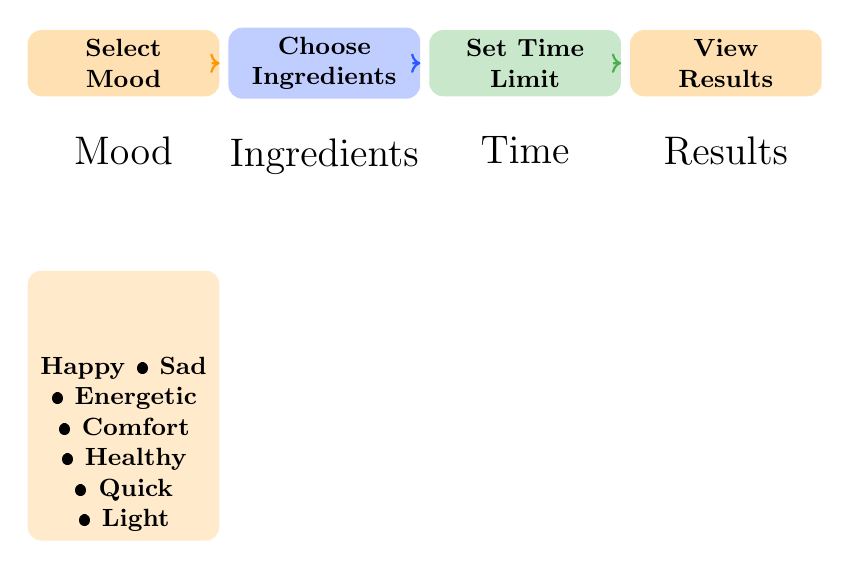
\begin{tikzpicture}[
        node distance=2cm,
        scale=0.85,
        every node/.style={rectangle, rounded corners=5pt, text centered, font=\small\bfseries}
    ]
        % Step 1
        \node[fill=Primary!30, text width=2.2cm] (step1) at (0, 6) {Select\\Mood};
        
        % Step 2
        \node[fill=Secondary!30, text width=2.2cm] (step2) at (3, 6) {Choose\\Ingredients};
        
        % Step 3
        \node[fill=Accent!30, text width=2.2cm] (step3) at (6, 6) {Set Time\\Limit};
        
        % Step 4
        \node[fill=Primary!30, text width=2.2cm] (step4) at (9, 6) {View\\Results};
        
        % Arrows
        \draw[->, thick, color=Primary, shorten >=3pt, shorten <=3pt] (step1) -- (step2);
        \draw[->, thick, color=Secondary, shorten >=3pt, shorten <=3pt] (step2) -- (step3);
        \draw[->, thick, color=Accent, shorten >=3pt, shorten <=3pt] (step3) -- (step4);
        
        % Icons below
        \node[below=0.5cm of step1, font=\Large, inner sep=0] {Mood};
        \node[below=0.5cm of step2, font=\Large, inner sep=0] {Ingredients};
        \node[below=0.5cm of step3, font=\Large, inner sep=0] {Time};
        \node[below=0.5cm of step4, font=\Large, inner sep=0] {Results};
        
        % Mood Emotions
        \node[below=2.2cm of step1, fill=Primary!20, text width=2.2cm, text height=1.2cm] {Happy • Sad • Energetic • Comfort • Healthy • Quick • Light};
    \end{tikzpicture}
    
    \vspace*{1.5cm}
    
    \begin{center}
        \includegraphics[width=0.7\textwidth]{\detokenize{../../Diagrams/sequence diagram recipe by mood.png}}
    \end{center}
\end{frame}

% ============================================================
% SLIDE 7: DESIGN PATTERNS & ARCHITECTURE
% ============================================================
\begin{frame}{Design Patterns \& Architecture}
    \vspace*{0.3cm}
    
    \begin{columns}[T]
        \column{0.48\textwidth}
        \centering
        \textcolor{Primary}{\textbf{\large Design Patterns}}
        
        \vspace{0.5cm}
        
        \begin{itemize}
            \item \textbf{Provider Pattern}\\State management
            \vspace{0.3cm}
            \item \textbf{Repository Pattern}\\Data abstraction
            \vspace{0.3cm}
            \item \textbf{Singleton Pattern}\\Shared instances
            \vspace{0.3cm}
            \item \textbf{Factory Pattern}\\Object creation
        \end{itemize}
        
        \column{0.48\textwidth}
        
        \centering
        \includegraphics[width=0.95\textwidth]{architecture-overview.png}
    \end{columns}
\end{frame}

% ============================================================
% SLIDE 8: DEPLOYMENT & DEVOPS
% ============================================================
\begin{frame}{Deployment \& DevOps Pipeline}
    \vspace*{0.5cm}
    
    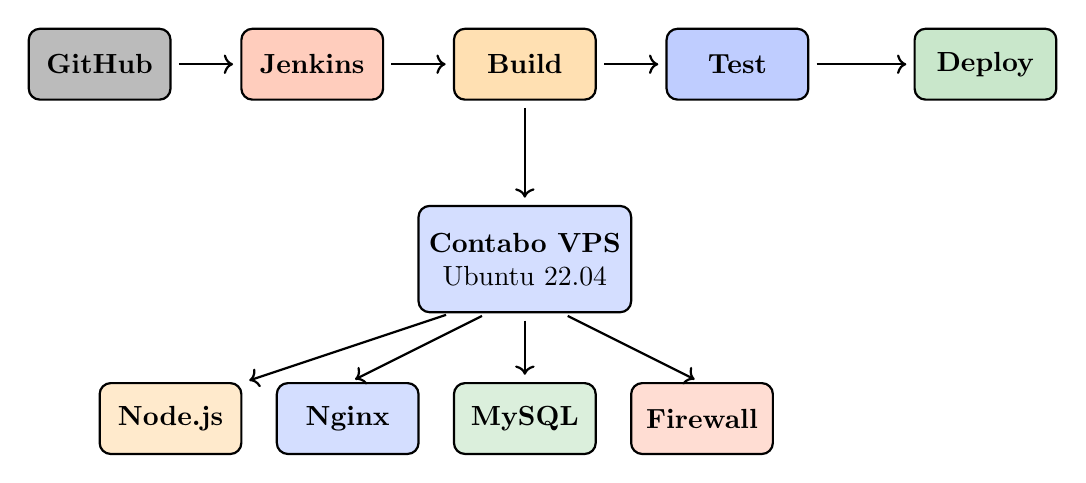
\begin{tikzpicture}[scale=0.9, thick]
        % GitHub
        \draw[fill=DarkBg!30, thick, rounded corners] (0, 5) rectangle (2, 6);
        \node at (1, 5.5) {\textbf{GitHub}};
        
        % Jenkins
        \draw[fill=Warning!30, thick, rounded corners] (3, 5) rectangle (5, 6);
        \node at (4, 5.5) {\textbf{Jenkins}};
        
        % Build
        \draw[fill=Primary!30, thick, rounded corners] (6, 5) rectangle (8, 6);
        \node at (7, 5.5) {\textbf{Build}};
        
        % Test
        \draw[fill=Secondary!30, thick, rounded corners] (9, 5) rectangle (11, 6);
        \node at (10, 5.5) {\textbf{Test}};
        
        % Arrows top
        \draw[->, thick, shorten >=3pt, shorten <=3pt] (2, 5.5) -- (3, 5.5);
        \draw[->, thick, shorten >=3pt, shorten <=3pt] (5, 5.5) -- (6, 5.5);
        \draw[->, thick, shorten >=3pt, shorten <=3pt] (8, 5.5) -- (9, 5.5);
        \draw[->, thick, shorten >=3pt, shorten <=3pt] (11, 5.5) -- (12.5, 5.5);
        
        % Deploy
        \draw[fill=Accent!30, thick, rounded corners] (12.5, 5) rectangle (14.5, 6);
        \node at (13.5, 5.5) {\textbf{Deploy}};
        
        % VPS
        \draw[fill=Secondary!20, thick, rounded corners] (5.5, 2) rectangle (8.5, 3.5);
        \node at (7, 2.75) [align=center] {\textbf{Contabo VPS}\\Ubuntu 22.04};
        
        % Services
        \draw[fill=Primary!20, thick, rounded corners] (1, 0) rectangle (3, 1);
        \node at (2, 0.5) {\textbf{Node.js}};
        
        \draw[fill=Secondary!20, thick, rounded corners] (3.5, 0) rectangle (5.5, 1);
        \node at (4.5, 0.5) {\textbf{Nginx}};
        
        \draw[fill=Accent!20, thick, rounded corners] (6, 0) rectangle (8, 1);
        \node at (7, 0.5) {\textbf{MySQL}};
        
        \draw[fill=Warning!20, thick, rounded corners] (8.5, 0) rectangle (10.5, 1);
        \node at (9.5, 0.5) {\textbf{Firewall}};
        
        % Arrows down
        \draw[->, thick, shorten >=3pt, shorten <=3pt] (7, 5) -- (7, 3.5);
        \draw[->, thick, shorten >=3pt, shorten <=3pt] (6, 2) -- (3, 1);
        \draw[->, thick, shorten >=3pt, shorten <=3pt] (6.5, 2) -- (4.5, 1);
        \draw[->, thick, shorten >=3pt, shorten <=3pt] (7, 2) -- (7, 1);
        \draw[->, thick, shorten >=3pt, shorten <=3pt] (7.5, 2) -- (9.5, 1);
    \end{tikzpicture}
    
    \vspace*{1cm}
    \centering
    \small \textcolor{gray}{\textbf{99.8\% Uptime} | CI/CD Automation | Real-time Monitoring}
\end{frame}

% ============================================================
% SLIDE 9: TESTING & METRICS
% ============================================================
\begin{frame}{Testing \& Quality Metrics}
    \vspace*{0.5cm}
    
    \begin{columns}[T]
        \column{0.48\textwidth}
        \centering
        \textcolor{Primary}{\textbf{\large Test Coverage}}
        
        \vspace{0.8cm}
        
        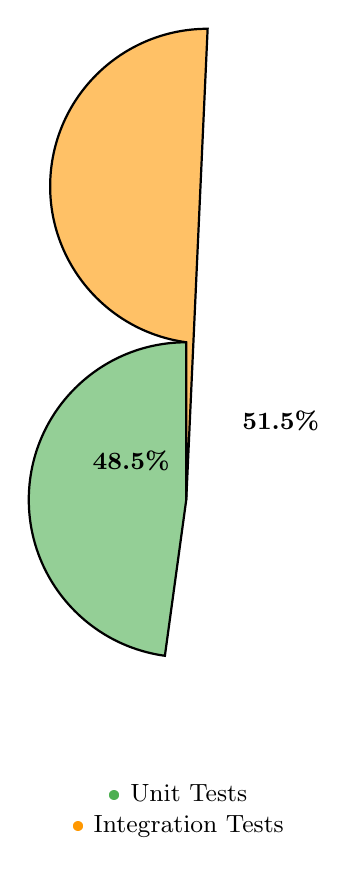
\begin{tikzpicture}[scale=1.0]
            % Pie chart representation
            \draw[fill=Accent!60, thick] (0,0) -- (0,2) arc[start angle=90, end angle=262.2, radius=2] -- cycle;
            \node at (-0.7, 0.5) {\small \textbf{48.5\%}};
            
            \draw[fill=Primary!60, thick] (0,0) -- (0,2) arc[start angle=262.2, end angle=90, radius=2] -- cycle;
            \node at (1.2, 1.0) {\small \textbf{51.5\%}};
            
            % Legend
            \node[below=1.5cm of current bounding box.south, text width=3cm, align=center, font=\small] {
                \textcolor{Accent}{\textbullet} Unit Tests\\
                \textcolor{Primary}{\textbullet} Integration Tests
            };
        \end{tikzpicture}
        
        \column{0.48\textwidth}
        \centering
        \textcolor{Secondary}{\textbf{\large Performance}}
        
        \vspace{0.5cm}
        
        \begin{tabularx}{0.95\textwidth}{|l|c|}
            \hline
            \rowcolor{Secondary!20}
            \textbf{Metric} & \textbf{Target} \\
            \hline
            Recipe Load Time & \textcolor{Accent}{\textbf{<2s}} \\
            \hline
            API Response & \textcolor{Accent}{\textbf{<500ms}} \\
            \hline
            Database Query & \textcolor{Accent}{\textbf{<300ms}} \\
            \hline
            Uptime & \textcolor{Accent}{\textbf{99.8\%}} \\
            \hline
        \end{tabularx}
    \end{columns}
\end{frame}

% ============================================================
% SLIDE 10: CONCLUSION & FUTURE ROADMAP
% ============================================================
\begin{frame}{Conclusion \& Future Roadmap}
    \vspace*{0.5cm}
    
    \begin{columns}[T]
        \column{0.48\textwidth}
        \centering
        \textcolor{Primary}{\textbf{\large Achievements}}
        
        \vspace{0.5cm}
        
        \begin{itemize}
            \item Fully functional cross-platform app
            \vspace{0.3cm}
            \item Secure authentication system
            \vspace{0.3cm}
            \item Offline-first architecture
            \vspace{0.3cm}
            \item Fast, responsive UI
            \vspace{0.3cm}
            \item Automated deployment
            \vspace{0.3cm}
            \item Comprehensive testing
        \end{itemize}
        
        \column{0.48\textwidth}
        \centering
        \textcolor{Secondary}{\textbf{\large Future Enhancements}}
        
        \vspace{0.5cm}
        
        \begin{itemize}
            \item AI-powered recommendations
            \vspace{0.3cm}
            \item Multi-language support
            \vspace{0.3cm}
            \item Advanced analytics
            \vspace{0.3cm}
            \item Smart notifications
            \vspace{0.3cm}
            \item Nutrition tracking
            \vspace{0.3cm}
            \item Social sharing
        \end{itemize}
    \end{columns}
    
    \vspace*{1.5cm}
    \centering
    \Large \textcolor{Primary}{\textbf{Making meal planning accessible, enjoyable, and efficient}}
\end{frame}

% ============================================================
% THANK YOU SLIDE
% ============================================================
\begin{frame}[plain]
    \begin{tikzpicture}[remember picture, overlay]
        \fill[color=Primary!5] (current page.south west) rectangle (current page.north east);
        \fill[color=Secondary!10] (current page.north west) -- (current page.north east) -- 
              ($(current page.north east)!0.4!(current page.south east)$) -- 
              ($(current page.north west)!0.4!(current page.south west)$) -- cycle;
    \end{tikzpicture}
    
    \centering
    \vspace*{2cm}
    
    {\Huge \textbf{\textcolor{Primary}{Thank You!}}}\\[1cm]
    
    {\Large \textcolor{Secondary}{Questions?}}\\[2cm]
    
    \includegraphics[width=0.2\textwidth]{app-logo.png}\\[1.5cm]
    
    {\small \faGithub\ \href{https://github.com/Kynmmarshall/Pick-My-Dish}{GitHub Repository}}\\
    {\small \faGlobe\ \href{https://pickmydish.duckdns.org}{Live Application}}\\[1.5cm]
    
    {\footnotesize \textcolor{gray}{ICT University - SEN3140 | January 2026}}
\end{frame}

\end{document}
